\chapter{Counting number of partitions into independent sets}
\label{chap:num-partitions-into-indep-sets}

\begin{highlight}

Important thing to note about results of table \ref{tab:platonic-exactly-n-clrs} above is the fact, that we count two colorings $c_1$ and $c_2$ as different also in the case, when $c_1$ can be obtained as a permutation of colors of $c_2$. This is something we would like to avoid if we are interested in the structure of the coloring only and the value of the colors bear no special meaning to us. 

\begin{defn}[relabeling relation]\label{dfn:relabeling-relation}
    Given a graph $G=(V,E)$ and a set of colorings $C$, we define a relation $\leftrightarrow \; \subseteq C \times C$ as follows: For any two colorings $c_1,c_2 \in C$ we have $c_1 \leftrightarrow c_2$ iff exists a permutation of colors $\pi$ s.t. $\forall v \in V : c_1(v) = \pi(c_2(v))$. We call this relation the \emph{relabeling relation}.
\end{defn}

The relabeling relation is in fact an equivalence relation as it is reflexive, symmetric and transitive.

\begin{defn}[number of exact n-partitions]
    Let us for a given $n \in \mathbb{N}$ denote by $P^*_{\leftrightarrow}(G,n)$ the number of equivalence classes of $\leftrightarrow$ on the set of all proper vertex colorings. 
\end{defn}

The equivalence classes in definition above correspond to different partitions of the set $V(G)$ into independent sets irrespectively of the particular colors that we assign the vertices. Note that now, we might still consider two partitions as different even though they can be made equal by applying some automorphism. In order to calculate $P^*_{\leftrightarrow}(G,n)$, consider any partition $W$ of $V(G)$ into independent sets and count how many different colorings correspond to $W$. Because $W$ consists of exactly $n$ independent sets, we have $n!$ possible ways of assigning colors to the independent sets of $W$. As this holds for any arbitrary partition of size $n$, it follows that:
\begin{equation}\label{eqn:count-relabel-orbits}
    P^*_{\leftrightarrow}(G,n) \cdot n! = P^*(G,n)
\end{equation}

Using this formula, we can compute yet another table shown below:

\begin{table}[H]
\centering
\begin{tabular}{l@{\hspace{0.5cm}}ccccccc}
\toprule
\textbf{Platonic solid} & \textbf{2} & \textbf{3} & \textbf{4} & \textbf{5} & \textbf{6} & \textbf{7} & \textbf{8} \\
\midrule
tetrahedron & $0$ & $0$ & $1$ & $0$ & $0$ & $0$ & $0$ \\
octahedron & $0$ & $1$ & $3$ & $3$ & $1$ & $0$ & $0$ \\
cube & $1$ & $18$ & $92$ & $146$ & $80$ & $16$ & $1$ \\
icosahedron & $0$ & $0$ & $10$ & $660$ & $4908$ & $10008$ & $7900$ \\
dodecahedron & $0$ & $1200$ & $7019920$ & $\approx 10^{8}$ & $\approx 10^{10}$ & $\approx 10^{11}$ & $\approx 10^{11}$ \\
\bottomrule
\end{tabular}
\caption{Numbers of of possible partitions of vertices of the graphs into $n$ independent sets.}
\label{tab:platonic-exact-n-partitions}
\end{table}

\vtodo{Add also evaluation for some of the Archimedean solids}

Notice, that even though we managed to overcome the problem of counting a single partition $W$ of $G$ into independent sets multiple times, because of the ways we can relabel the colorings, the method still suffers from the following: Rotated or reflected independent sets might be counted as different objects. This happens exactly in the cases, when by rotating some partition $W_1$, we arrive at a partition $W_2$ s.t. for any coloring $c_1$ obtained by labeling the sets of $W_1$ and for any coloring $c_2$ obtained by labeling sets of $W_2$ we have $c_1 \not\leftrightarrow c_2$. In other words, we cannot create $c_2$ by renaming the colors of $c_1$ or vice versa.

This problem is illustrated on figure \ref{fig:example-octahedron-4-partitions} below. We can see that all three partitions are same when we allow rotating the solid. But it is impossible to arrive from one coloring to another by simply relabeling the colors. 

\begin{figure}[H]
    \centering
    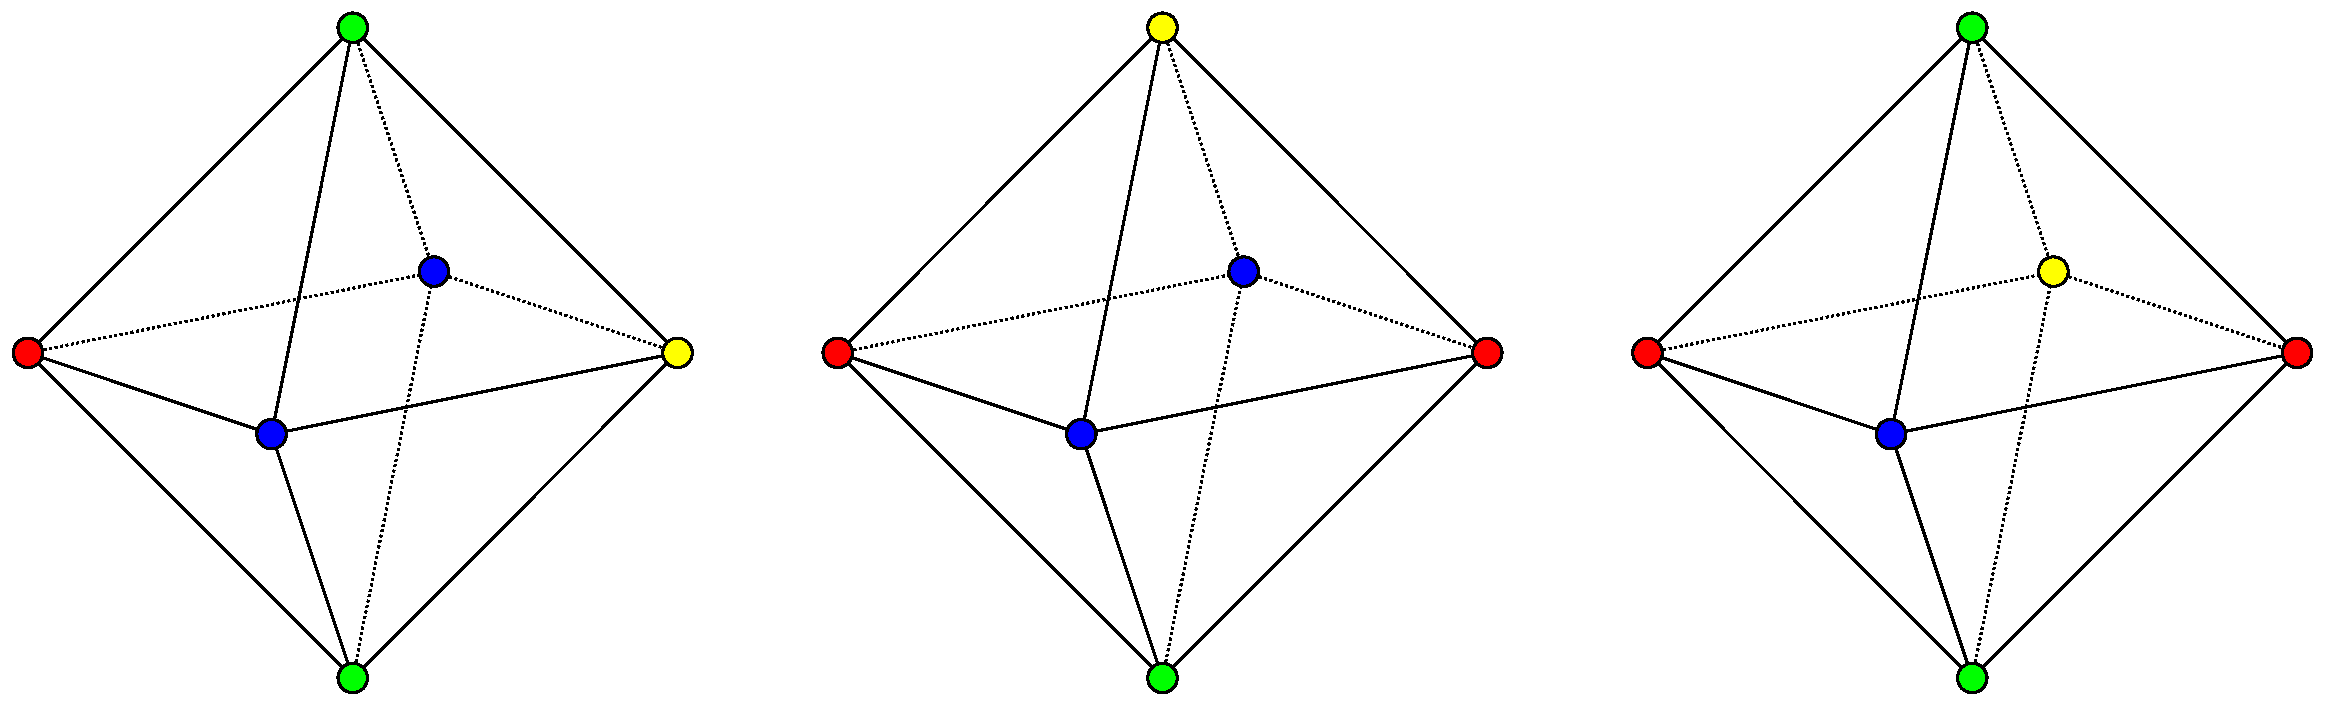
\includegraphics[width=1\textwidth]{Resources/Figs/example-octahedron-4-partitions.pdf}
    \caption{All partitions of octahedron to 4 independent sets. Notice that they are structurally the same partitions when we allow us to rotate the solid.}
    \label{fig:example-octahedron-4-partitions}
\end{figure}

Note that in some cases of symmetric colorings, this problem is avoided. For example, any rotation or reflection of a 4-coloring of tetrahedron can be obtained by simply relabeling the colors as well. See this on the figure below:

\begin{figure}[H]
    \centering
    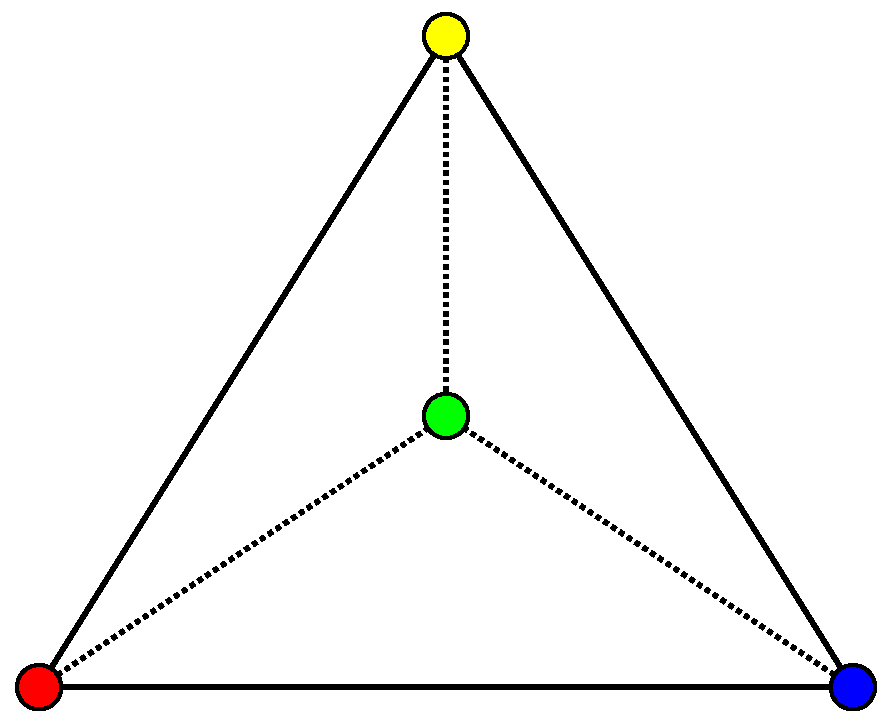
\includegraphics[width=0.3\textwidth]{Resources/Figs/example-tetrahedron-4-clring.pdf}
    \caption{A coloring of tetrahedron using 4 colors. Notice that any rotation of this coloring can be obtained by simply relabeling the colors.}
    \label{fig:example-tetrahedron-4-coloring}
\end{figure}

Overcoming the problem of counting rotations or reflection of the same partition multiple times motivates the following definition:

\begin{defn}[relabeling-automorphism relation]\label{dfn:relabeling-automorphism-relation}
    Let $G=(V,E)$ be a graph and $C$ a set of its vertex colorings. We define a relation $\rightleftharpoons \; \subseteq C \times C$ as follows: Given two colorings $c_1,c_2 \in C$ we have $c_1 \rightleftharpoons c_2$ iff there exists a permutation of colors $\pi$ and an automorphism $\alpha \in \Aut(G)$ s.t. $\forall v \in V : c_1(v) = \pi(c_2(\alpha(v)))$. We call this relation the \emph{relabeling-automorphism relation}.
\end{defn}

The relabeling-automorphism relation is again an equivalence relation. For reflexivity, we can simply take $\pi = id$ and $\alpha = id$. For symmetry, suppose we have $\pi$ and $\alpha$ s.t. $\forall v \in V : c_1(v) = \pi(c_2(\alpha(v)))$. Suppose we have a $w \in V$, then there exists $v \in V$ s.t. $w = \alpha(v)$. We will show that $c_2(w) = \pi^{-1}(c_1(\alpha^{-1}(w)))$. We can rewrite the previous in form $c_2(\alpha(v)) = \pi^{-1}(c_1(\alpha^{-1}(\alpha(v))))$ which is equivalent to $c_2(\alpha(v)) = \pi^{-1}(c_1(v)) \iff c_1(v) = \pi(c_2(\alpha(v)))$ which holds by the assumption. For transitivity, we have that $\exists \pi, \pi', \alpha ,\alpha'$ s.t. $\forall v \in V : c_1(v) = \pi(c_2(\alpha(v))) \wedge c_2(v) = \pi'(c_3(\alpha'(v)))$ from which we get $c_1(v)=\pi(\pi'(c_3(\alpha'(\alpha(v)))))$. This means that $\pi \circ \pi'$ and $\alpha' \circ \alpha$ are the permutation of colors and automorphism we are looking for.

Since $\rightleftharpoons$ is an equivalence relation, we can again consider its partition into equivalence classes, $C/_\rightleftharpoons$ and count the number of these classes, $\abs{C/_\rightleftharpoons}$. This is be an interesting number to calculate, since if $C$ is the set of n-colorings of graph $G$, then each equivalence class corresponds to a structurally different partitioning of $G$ into $n$ non-empty independent sets.

\begin{defn}[orbital number of exact n-partitions]
    Let us for a given $n \in \mathbb{N}$ denote by $P^*_{\rightleftharpoons}(G,n)$ the number of equivalence classes of $\rightleftharpoons$ on the set of all proper vertex colorings. 
\end{defn}

It is tempting to suppose that $P^*_{\rightleftharpoons}(G,n)$ can be calculated from $OP^*(G,n)$ in a similar fashion as can be $P^*_{\leftrightarrow}(G,n)$ calculated using $P^*(G,n)$ by formula \ref{eqn:count-relabel-orbits}. In that formula, we showed for each equivalence class of $C/_\leftrightarrow$, we count exactly $n!$ colorings in $C$ when we use $P^*(G,n)$. If something similar is to hold for $\rightleftharpoons$, we would have to show that for each equivalence class of $C/_\rightleftharpoons$, we count exactly $k$ equivalence classes of $C/_\sim$ when using $OP^*(G,n)$ for some fixed number $k$. Unfortunately, this is not the case since there exists graph $G$ and a set of its n-colorings $C$ s.t. there are equivalence classes of $C/_\rightleftharpoons$ that are counted exactly once by $OP^*(G,n)$ but also classes that are counted multiple times.

For example consider the graph of cube and its following two 4-colorings:

\begin{figure}[H]
    \centering
    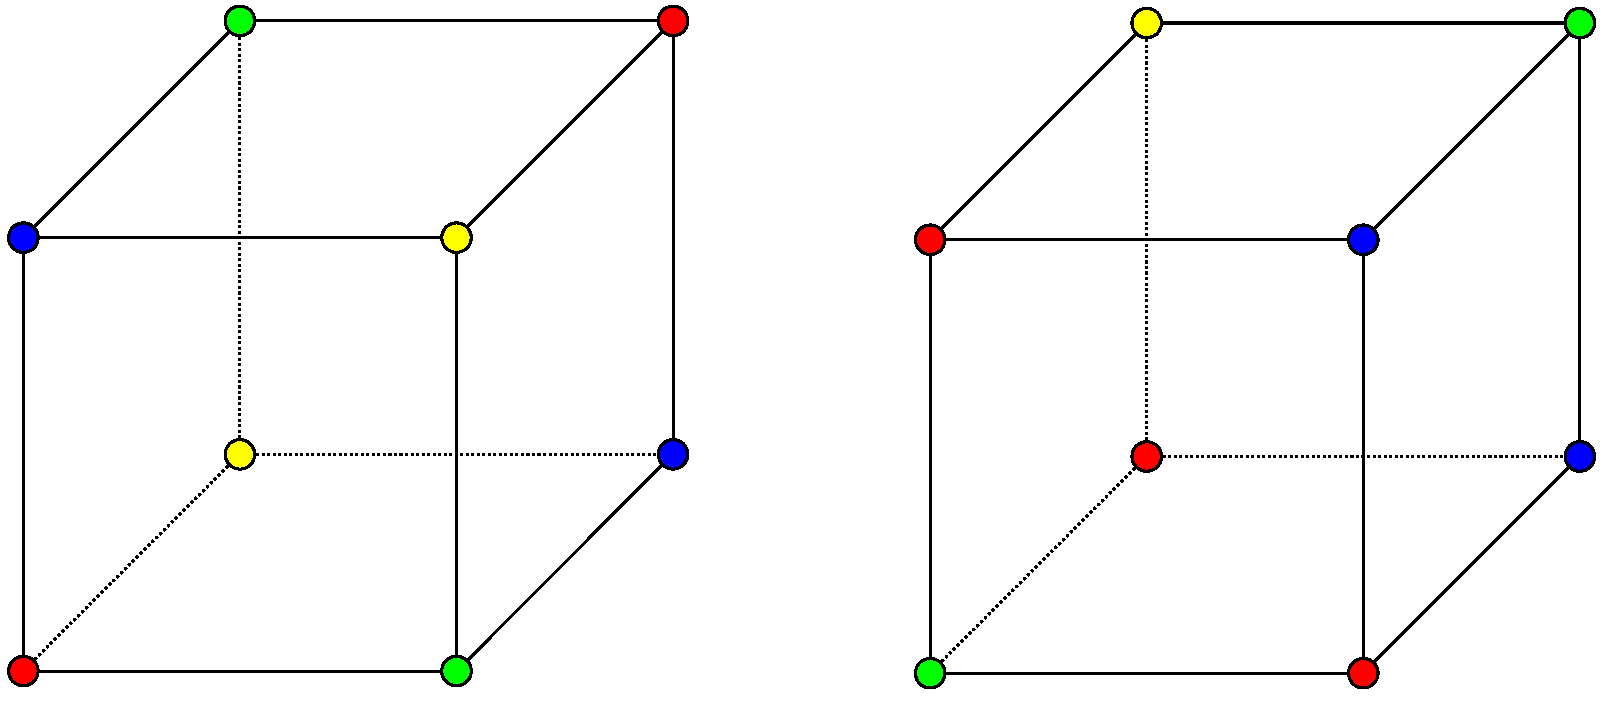
\includegraphics[width=0.75\textwidth]{Resources/Figs/example_diff_rel-aut_class_sizes.pdf}
    \caption{Two structurally different partitions of cube into independent sets.}
    \label{fig:example-cube-4-clrings-diff-classes}
\end{figure}

When the colorings in figure \ref{fig:example-cube-4-clrings-diff-classes} are viewed as a partition, then the left partition represents a single equivalence class of both $\sim$ and $\rightleftharpoons$. This follows from the fact, that permuting the colors of the independent set leads to a coloring, that can be obtained from the original coloring by simply rotating the solid.

On the other hand the partition one the right represents $4!$ equivalence classes of $\sim$ since any permutation of colors yields a different equivalence class of $\sim$.

\section{Simple bounds on number of equivalence classes of the relabeling-automorphism relation}

Before we show, how the number of equivalence classes of $\rightleftharpoons$ can be computed using a brute force algorithm, we provide bounds on the this number, $P^*_\rightleftharpoons(G,n)$, using the numbers $P^*_\leftrightarrow(G,n)$ and $OP^*(G,n)$.

\begin{claim}\label{clm:relabeling-bound}
    For any graph $G=(V,E)$ and a natural number $n$, we have: $$\frac{1}{\abs{\Aut(G)}} \cdot P^*_\leftrightarrow(G,n) \leq P^*_\rightleftharpoons(G,n) \leq P^*_\leftrightarrow(G,n)$$ 
\end{claim}

\begin{proof}

The inequality $P^*_\rightleftharpoons(G,n) \leq P^*_\leftrightarrow(G,n)$ is simple. It follows from the fact, that for any two colorings $c_1$,$c_2$ of graph $G$, if we have $c_1 \not\rightleftharpoons c_2$, then also $c_1 \not\leftrightarrow c_2$. So there must be at least as many equivalence classes of $\leftrightarrow$ as they are of $\rightleftharpoons$.

For inequality $\frac{1}{\abs{\Aut(G)}} \cdot P^*_\leftrightarrow(G,n) \leq P^*_\rightleftharpoons(G,n)$ we show, that for each equivalence class of $\rightleftharpoons$ there are at most $n!$ equivalence classes of $\leftrightarrow$. Remember that $n$ is the number of colors or independent sets that the colorings of $G$ we consider have. Let $c_1$ be some coloring, that belongs to some equivalence class $E_\rightleftharpoons$ of $\rightleftharpoons$ and equivalence class $E_\leftrightarrow$ of $\leftrightarrow$. All possible relabelings of colors of $c_1$ will be contained in both classes $E_\rightleftharpoons$ and $E_\leftrightarrow$. On the other hand, there exist at most $\abs{\Aut(G)}$ ways to rotate the coloring $c_1$ which will all be contained in $E_\rightleftharpoons$ but may result in at most $\abs{\Aut(G)}$ different equivalence classes of $\leftrightarrow$.

\end{proof}

Notice, that the result of claim $\ref{clm:relabeling-bound}$ gives us equality for any graph $G$ s.t. $\Aut(G) = \{id\}$ i.e. a graph, whose only symmetry is the identity function. In general, the lower bound is higher for graphs that are not very symmetric. Unfortunately, this is not the case for our graphs, so the lower bounds will not give us as much information.

Calculated values using these bounds are shown on table below:

\begin{table}[H]
\centering
\begin{tabular}{l@{\hspace{0.5cm}}ccccccc}
\toprule
\textbf{Platonic solid} & \textbf{2} & \textbf{3} & \textbf{4} & \textbf{5} & \textbf{6} & \textbf{7} & \textbf{8} \\
\midrule
tetrahedron & $0$ & $0$ & $1$ & $0$ & $0$ & $0$ & $0$ \\
 & $0$ & $0$ & $1$ & $0$ & $0$ & $0$ & $0$ \\
\specialrule{0.2pt}{0.65ex}{0.65ex}
octahedron & $0$ & $1$ & $3$ & $3$ & $1$ & $0$ & $0$ \\
 & $0$ & $1$ & $1$ & $1$ & $1$ & $0$ & $0$ \\
\specialrule{0.2pt}{0.65ex}{0.65ex}
cube & $1$ & $18$ & $92$ & $146$ & $80$ & $16$ & $1$ \\
 & $1$ & $1$ & $2$ & $4$ & $2$ & $1$ & $1$ \\
\specialrule{0.2pt}{0.65ex}{0.65ex}
icosahedron & $0$ & $0$ & $10$ & $660$ & $4908$ & $10008$ & $7900$ \\
 & $0$ & $0$ & $1$ & $6$ & $41$ & $84$ & $66$ \\
\specialrule{0.2pt}{0.65ex}{0.65ex}
dodecahedron & $0$ & $1200$ & $7019920$ & $\approx 10^{8}$ & $\approx 10^{10}$ & $\approx 10^{11}$ & $\approx 10^{11}$ \\
 & $0$ & $10$ & $58500$ & $7761169$ & $\approx 10^{8}$ & $\approx 10^{9}$ & $\approx 10^{9}$ \\
\bottomrule
\end{tabular}
\caption{Upper and lower bounds for the number of equivalence classes of the relabeling-automorphism relation based on the number of equivalence classes of the relabeling relation.}
\label{tab:bounds-exactn-n-partitions}
\end{table}

\begin{claim}\label{clm:automorphism-bound}
    For any graph $G=(V,E)$ and a natural number $n$, we have: $$\frac{1}{n!} \cdot OP^*(G,n) \leq P^*_\rightleftharpoons(G,n) \leq OP^*(G,n)$$
\end{claim}

\begin{proof}

Argument for inequality $P^*_\rightleftharpoons(G,n) \leq OP^*(G,n)$ is again simple and analogous to the one in clam \ref{clm:relabeling-bound}. We notice, that if for any two colorings $c_1,c_2$ we have $c_1 \not\rightleftharpoons c_2$ then also $c_1 \not\sim c_2$.

For inequality $\frac{1}{n!} \cdot OP^*(G,n) \leq P^*_\rightleftharpoons(G,n)$ we proceed again analogously as in claim \ref{clm:relabeling-bound}. We show that for each equivalence class of $\rightleftharpoons$ we have at most $n!$ equivalence classes of $\sim$. We imagine a coloring $c_1$ that belongs to some equivalence class $E_\rightleftharpoons$ of $\rightleftharpoons$ and $E_\sim$ of $\sim$. Applying any automorphism $\alpha \in \Aut(G)$ results in a coloring, that will be contained in both $E_\rightleftharpoons$ and $E_\sim$. On the other hand, by relabeling the colors of $c_1$ we may obtain $n!$ colorings s.t. each belongs to a different equivalence class of $\sim$ even though they all belong to $E_\rightleftharpoons$.

\end{proof}

Note, that the lower bound resulting from claim $\ref{clm:automorphism-bound}$ is useful for cases where $n$, the number of colors, is small. In such cases, it can give us a better bound than what the bound from claim $\ref{clm:relabeling-bound}$ gives.

See values resulting from this bound in the table below and compare with table \ref{tab:bounds-exactn-n-partitions}.

\begin{table}[H]
\centering
\begin{tabular}{l@{\hspace{0.5cm}}ccccccc}
\toprule
\textbf{Platonic solid} & \textbf{2} & \textbf{3} & \textbf{4} & \textbf{5} & \textbf{6} & \textbf{7} & \textbf{8} \\
\midrule
tetrahedron & $0$ & $0$ & $1$ & $0$ & $0$ & $0$ & $0$ \\
 & $0$ & $0$ & $1$ & $0$ & $0$ & $0$ & $0$ \\
\specialrule{0.2pt}{0.65ex}{0.65ex}
octahedron & $0$ & $1$ & $6$ & $15$ & $15$ & $0$ & $0$ \\
 & $0$ & $1$ & $1$ & $1$ & $1$ & $0$ & $0$ \\
\specialrule{0.2pt}{0.65ex}{0.65ex}
cube & $1$ & $12$ & $100$ & $485$ & $1290$ & $1680$ & $840$ \\
 & $1$ & $2$ & $5$ & $5$ & $2$ & $1$ & $1$ \\
\specialrule{0.2pt}{0.65ex}{0.65ex}
icosahedron & $0$ & $0$ & $2$ & $660$ & $29454$ & $420336$ & $2654400$ \\
 & $0$ & $0$ & $1$ & $6$ & $41$ & $84$ & $66$ \\
\specialrule{0.2pt}{0.65ex}{0.65ex}
dodecahedron & $0$ & $75$ & $1404548$ & $\approx 10^{8}$ & $\approx 10^{11}$ & $\approx 10^{12}$ & $\approx 10^{14}$ \\
 & $0$ & $13$ & $58523$ & $7761220$ & $\approx 10^{8}$ & $\approx 10^{9}$ & $\approx 10^{9}$ \\
\bottomrule
\end{tabular}
\caption{Upper and lower bounds for the number of equivalence classes of the relabeling-automorphism relation based on the number of equivalence classes of the $\sim$ relation.}
\label{tab:bounds-orbital}
\end{table}

\vtodo{Demonstrate the bound on the example of dodecahedron}

\section{Algorithm for computing number of equivalence classes of the relabeling-automorphism relation}

For all the algorithms below, we assume that we are working with colorings using $n$ colors. The colorings are represented as lists of integers ranging from $0$ to $n-1$, where $n$ is the number of colors. The lists are indexed by vertices, which are numbers $0, \ldots,|V|-1$.

Since we are dealing with graphs that have relatively small amount of edges and vertices, we can compute some of the numbers using a simple algorithm that works by first enumerating all coloring and then filtering the ones that are equivalent. The algorithm can be split into the following two parts:

\subsection{Finding representatives of the relabeling relation}

First, we want to exclude colorings, that correspond to the same partitions into independent sets, but just have different labels for the colors. This corresponds to finding colorings that represent different classes of the relabeling relation from definition \ref{dfn:relabeling-relation}. We use the fact, that the colorings are represented as lists together with the following observation: Given a partition into $n$ independent sets, there are $n!$ ways to assign labels to the colorings. Out of these $n!$ colorings, there will be always exactly one of them s.t. the coloring is in a so called \textit{canonic form}.  

\begin{defn}\label{dfn:canonic-form}
    Let $B=\{0,\ldots,n-1\}$ be a set of colors and $c$ be a coloring using colors from $B$ s.t. $c$ is represented as sequence $(b_0, \ldots,b_{\abs{V}-1})$ s.t. $\forall i: b_i \in B$. For each $i \in B$ denote $k_i$ the lowest index at which color $i$ appears. We say that $c$ is in \emph{canonic form} if $\forall i < j \in B: k_i < k_j$.
\end{defn}

In other words, a coloring is in canonic form ,if when we go through the coloring from lowest index to highest index, we encounter the colors for the first time in the same order as what the values of the colors are. Now the observation is, that for all $n!$ relabelings of the independent sets, there is exactly one coloring s.t. it is in canonic form. This means, that by keeping only the colorings in canonic form, we get exactly colorings representing the equivalence classes of the relabeling relation.

\begin{algorithm}[H]
    \caption{Algorithm for testing that a given coloring is in canonic form as in definition \ref{dfn:canonic-form}} 
    \begin{algorithmic}[1]
        \Function{IsInCanonicForm}{$c$}
            \State $k \gets 0$      
            \For{color $b_i$ in coloring $c$}
                \If{$b_i > k$}
                    \State \Return False
                \EndIf
                 \If{$b_i = k$}
                    \State $k \gets k + 1$
                \EndIf
            \EndFor   
            \State \Return True
        \EndFunction
    \end{algorithmic}
    \label{alg:is-in-canonic-form}
\end{algorithm}

\subsection{Finding representatives of relabeling-automorphism relation}

By filtering the colorings that are not in canonic form, we have reduced the number of colorings we need to deal with by a factor of $n!$. After doing that, we can proceed with a more computationally heavy part of the algorithm. In this part of the algorithm, we run through all the colorings and build a set $R$ of representatives of the relabeling-automorphism class. In each step, when we consider some next coloring $c_i$, we compare $c_i$ with all representatives in $R$. If $c_i$ can be unified by an automorphism with some representative $r_j \in R$, then we continue to the next coloring. Otherwise, we add $c_i$ to $R$ i.e. we declare $c_i$ as a representative of its class. See detailed description of the algorithm below:

\begin{algorithm}[H]
    \caption{Algorithm for finding representatives of relabeling-automorphism relation as defined in \ref{dfn:relabeling-automorphism-relation}} 
    \begin{algorithmic}[1]
        \Function{FindRelabelingAutomorphismRepresentatives}{$G,C$}
            \State $R \gets \emptyset$
            \For{coloring $c_i \in C$}
                \For{coloring $r_j \in R$}
                    \If{$c_i$ and $c_j$ can be unified by some $\alpha \in \Aut(G)$ and relabeling}
                        \State Continue with next coloring at step 3
                    \EndIf
                \EndFor
                \State $R \gets R \cup \{c_i\}$
            \EndFor
            \State \Return $R$
        \EndFunction
    \end{algorithmic}
    \label{alg:representatives-of-relabeling-automorphism-relation}
\end{algorithm}

Using this algorithm, we can just ask for size of set $R$ to get the number of equivalence classes of the $\rightleftharpoons$ relation. Since step $5$ of the algorithm above is a bit more involved, we describe it in more detail below. We use notation $\Dom(f)$ and $\Rng(f)$ to describe domain and range of function $f$ respectively. Also we treat each cycle $O$ of an automorphism $\alpha$ as a sequence of vertices $(v_1,\ldots,v_k)$ where $k := \abs{O}$. See the description of the algorithm below:

\begin{algorithm}[H]
    \caption{Algorithm testing if two colorings $c_1, c_2$ can be unified by given automorphism $\alpha$ by some relabeling.} 
    \begin{algorithmic}[1]
        \Function{TestRelabelingAutomorphismRelated}{$c_1,c_2,\alpha$}
            \State $f \gets \emptyset$
            \For{cycle $O \in \alpha$}
                \State $k \gets \abs{O}$
                \For{$v_i \in O$}
                    \If{$c_1(v_i ) \notin \Dom(f)$}
                        \If{$c_2(v_{i + 1 \bmod k}) \notin \Rng(f)$}
                            \State $f(c_1(v_i)) \gets c_2(v_{i + 1 \bmod k})$
                        \Else
                            \State \Return False
                        \EndIf
                    \Else
                        \If{$f(c_1(v_i )) \neq c_2(v_{i + 1 \bmod k})$}
                            \State \Return False
                        \EndIf
                    \EndIf
                \EndFor
            \EndFor
            \State \Return True
        \EndFunction
    \end{algorithmic}
    \label{alg:test-two-colorings-relabel-automorph-related}
\end{algorithm}

In natural language, the algorithm above tries to construct a mapping $f$ from colors of coloring $c_1$ to colors of coloring $c_2$. This mapping must be a valid permutation of colors, so we require that no two colors from $c_1$ map to a single color in $c_2$.

Step $5$ of algorithm \ref{alg:representatives-of-relabeling-automorphism-relation} consists of testing, whether for some $\alpha \in \Aut(G)$, the algorithm \ref{alg:test-two-colorings-relabel-automorph-related} above returns true.

See next section for results we computed using the algorithm above.

\section{Numbers of equivalence classes of relabeling-automorphism relation}

\begin{table}[H]
\centering
\begin{tabular}{l@{\hspace{0.5cm}}ccccccc}
\toprule
\textbf{Platonic solid} & \textbf{2} & \textbf{3} & \textbf{4} & \textbf{5} & \textbf{6} & \textbf{7} & \textbf{8} \\
\midrule
tetrahedron & $0$ & $0$ & $1$ & $0$ & $0$ & $0$ & $0$ \\
octahedron & $0$ & $1$ & $1$ & $1$ & $1$ & $0$ & $0$ \\
cube & $1$ & $3$ & $9$ & $10$ & $7$ & $2$ & $1$ \\
icosahedron & $0$ & $0$ & $1$ & $12$ & $\cdot$ & $\cdot$ & $\cdot$ \\
dodecahedron & $0$ & $17$ & $\cdot$ & $\cdot$ & $\cdot$ & $\cdot$ & $\cdot$ \\
\bottomrule
\end{tabular}
\caption{Calculated numbers of equivalence classes of the $\rightleftharpoons$ relation of Platonic solids using the algorithm above. The symbol $\cdot$ means that the computation took longer than 60 seconds and hence was terminated.}
\label{tab:plat-nums-relabeling-automorphism-classes}
\end{table}

\begin{table}[H]
\centering
\begin{tabular}{l@{\hspace{0.5cm}}ccccccc}
\toprule
\textbf{Archimedean solid} & \textbf{2} & \textbf{3} & \textbf{4} & \textbf{5} & \textbf{6} & \textbf{7} & \textbf{8} \\
\midrule
truncated tetrahedron & $0$ & $2$ & $119$ & $\cdot$ & $\cdot$ & $\cdot$ & $\cdot$ \\
cuboctahedron & $0$ & $2$ & $24$ & $\cdot$ & $\cdot$ & $\cdot$ & $\cdot$ \\
truncated cube & $0$ & $65$ & $\cdot$ & $\cdot$ & $\cdot$ & $\cdot$ & $\cdot$ \\
truncated octahedron & $1$ & $\cdot$ & $\cdot$ & $\cdot$ & $\cdot$ & $\cdot$ & $\cdot$ \\
\bottomrule
\end{tabular}
\caption{Calculated numbers of equivalence classes of the $\rightleftharpoons$ relation of selected Archimedean solids using the algorithm above. The symbol $\cdot$ means that the computation took longer than 60 seconds and hence was terminated.}
\label{tab:arch-nums-relabeling-automorphism-classes}
\end{table}

\vtodo{Show colorings corresponding to some of the entries in the tables above}

\end{highlight}